\subsection{XOR}
    The XOR gate, short for Exclusive OR, represents the expression $(A\cdot {\overline {B}})+({\overline {A}}\cdot B)$.
    It can be constructed using AND, OR and NOT gates, however, this approach would require five gates of three different kinds. 
    As an alternative, the XOR gate can be made of just universal gates, such as NAND or NOR gates: from four NAND gates, as shown in Figure \ref{fig:XOR_gate1}, or from five NOR gates, as shown in Figure \ref{fig:XOR_gate2}. \\\\	
    \begin{figure}[H]   
        \begin{minipage}{0.5\textwidth}
            \centering
            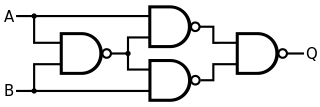
\includegraphics[width=0.8\textwidth]{figures/circuits/XOR1.png}
            \captionof{figure}{XOR gate from NAND gates.} 
            \label{fig:NOR_gate1} 
        \end{minipage}
        \begin{minipage}{0.5\textwidth}
            \centering
            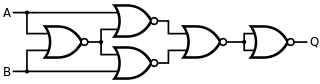
\includegraphics[width=1\textwidth]{figures/circuits/XOR2.png}
            \captionof{figure}{XOR gate from NOR gates.} 
            \label{fig:NOR_gate2} 
        \end{minipage}
	\end{figure}
    
    \noindent
    % It produces an output of 0 when the number of input 1s is even. \\
    % The XOR gate is particularly useful for detecting changes in binary values and implementing binary addition. \\
    % The circuitry of an XOR gate involves a combination of AND, OR, and NOT gates, as shown in Figure \ref{fig:XOR_circuit}. \\
    % A XOR gate consists of multiple stages:
    % the first stage is an arrangement of AND gates, which evaluate the conditions where one input is 1 while the other is 0;
    % the second stage involves an OR gate, which combines the outputs of the AND gates;
    % finally, a NOT gate is sometimes added to invert the final output.\\
    % The XOR gate works by evaluating the two inputs. If the inputs are different (one is 0 and the other is 1), the AND gates in the first stage produce 0 outputs, resulting in a 1 output from the OR gate. 
    % If both inputs are the same (both 0 or both 1), the AND gates produce a 0 output, leading to a 0 output from the OR gate. 
    This behavior is consistent with the XOR gate's truth table shown in Table \ref{tab:XOR_table}. \\

    \begin{table}[ht]
        \centering
        \begin{tabular}{|c|c|c|}
            \hline
            Input A & Input B & Output \\
            \hline
            0 & 0 & 0 \\
            0 & 1 & 1 \\
            1 & 0 & 1 \\
            1 & 1 & 0 \\
            \hline
        \end{tabular}
        \caption{XOR truth table.}
        \label{tab:XOR_table}
    \end{table}   
    
    \begin{figure}[H]
	    \centering
	    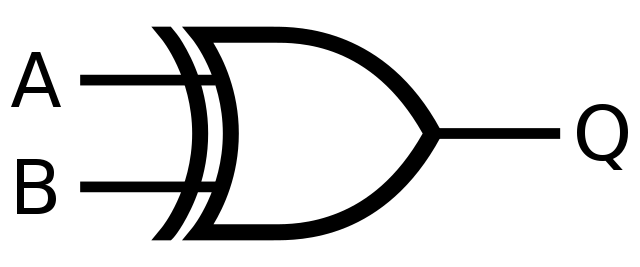
\includegraphics[width=0.3\textwidth]{figures/symbols/XOR.png}
	    \caption{XOR symbol.}
	    \label{fig:XOR_sym} 
	\end{figure}